\documentclass[3p]{elsarticle} %preprint/3p

\usepackage{hyperref}

\journal{   }
\usepackage[T1]{fontenc}
\usepackage{amsmath} %added for maths environments (equation and align)
\usepackage{amssymb}
\usepackage{upgreek}
\usepackage{bm} %bold symbols by using \bm
\usepackage{mathtools, nccmath} %added for \xrightleftharpoons
\usepackage{stmaryrd} %math symbols
\usepackage{subcaption} %allowing for subcaptions and subfigures
\captionsetup[sub]{font=normalsize}%normalsize

\usepackage{algorithm} %added for algorithm box
\usepackage{algpseudocode}
\biboptions{sort&compress}

\usepackage[autostyle]{csquotes}
\MakeOuterQuote{"}

\bibliographystyle{elsarticle-num}

% slightly altering rules for figure placement to prevent full-page figures
\usepackage{placeins}
\renewcommand{\floatpagefraction}{.90}
\renewcommand{\topfraction}{.90}

\usepackage[capitalise, nameinlink]{cleveref}

\usepackage{todonotes} %added for todo notes
\let\oldtodo\todo
\renewcommand{\todo}[1]{\oldtodo[inline]{#1}}
%\renewcommand{\todo}[1]{\oldtodo[color=white!40,inline]{#1}}
\newcommand{\toask}[1]{\oldtodo[color=green!40, inline]{#1}}
\newcommand{\wrn}[1]{\oldtodo[color=red!40, inline]{#1}}
\setcounter{tocdepth}{2}
\usepackage{xcolor}
\usepackage{listings}
\usepackage{lstautogobble}
\usepackage[numbered]{matlab-prettifier}
\lstdefinestyle{mystyle}{
	numbers=left,
	numberstyle=\footnotesize,
	numbersep=8pt,
	style=Matlab-editor,
	tabsize=4,
	basicstyle=\ttfamily\footnotesize,
	numbersep=12pt,
	frame=none,
	autogobble=true
}
\newcommand{\CodeSnipU}[4]{\lstinputlisting[firstnumber=#2,firstline=#2,lastline=#3,style=mystyle,title={#4}]{../#1}}
\newcommand{\CodeSnip}[3]{\lstinputlisting[firstnumber=#2,firstline=#2,lastline=#3,style=mystyle,title={#1}]{../#1}}

\newcommand{\citeMe}{\href{https://doi.org/}{T Hageman. \textit{Phase-field fracture modelling of ice: From triaxial tests to ice-cliff collapse}. Computer Methods in Applied Mechanics and Engineering \citep{Hageman2025}}}

\begin{document}
\pagenumbering{gobble}
\begin{frontmatter}
\title{
\includegraphics[width=4cm,trim={0 180 0 0}]{../Physics/Visualisation/Icon.png} IceFEM: A finite element code to simulate fracture and viscous/plastic deformation in ice.}

\author{Tim Hageman \corref{mycorrespondingauthor}}
\cortext[mycorrespondingauthor]{Corresponding author}
\ead{tim.hageman@eng.ox.ac.uk}

\address{Department of Engineering Science, University of Oxford, Oxford OX1 3PJ, UK}
\begin{abstract}
Documentation that accompanies the \textit{C++} code \href{https://github.com/T-Hageman/Ice_FEM_2025a}{IceFEM, available from \textcolor{blue}{here}}. This documentation explains how to compile the code, the usage of the implemented finite element framework, and highlight the main files.  The code allows the simulation of the detailed failure behaviour of ice, considering brittle fractures through the phase-field model, capturing shear bands through von Mises plasticity, and capturing creep through Glens law. Several example files are also included, demonstrating how to set up the simulation of a tri-axial compression sample, and of an ice-cliff failure study. If using (part of) this code, please cite \citeMe{}.  
\end{abstract}

\begin{keyword}
Glaciology, Finite elements, Phase-field fracture, Plasticity, Ice mechanics
\end{keyword}

\end{frontmatter}

% \begin{figure}
% 	\centering
% 	\includegraphics[width=10cm]{Fig1.eps}
% 	\caption{Overview of the system simulated using the presented C++ code}
% \end{figure}

\tableofcontents

\newpage
\pagenumbering{arabic}
\section{Introduction}




\subsection{Installation}

\subsubsection{Required external libraries}
The simulation code has been developed to work directly in ubuntu, or within windows using WSL \citep{mattwojo}. A script is included which installs all required libraries, \textit{Install\_ICEFEM.sh}. While it can be directly run to install and compile all libraries at once, it is strongly recommended that the contents is run line-by-line by copying it into the terminal. This allows for easier debugging in case of errors. The following libraries are required:

\noindent \textbf{Intel OneMKL} \citep{oneMKL} is used for its linear matrix solvers (and used by PETSc).\\
\textbf{Eigen} \citep{eigen} is used for small matrix and vector mutliplications.\\
\textbf{RapidJSON} \citep{rapidjson} is used for reading the input files.\\
\textbf{VTK} \citep{VTK} is used for visualisation during simulations.\\
\textbf{Highfive} \citep{HighFive} is used to write output files in the HDF5 format.\\
\textbf{PETSc} \citep{PETSc} is used for its implementation of parrallel (MPI) matrices and vectors (and their associated solvers).\\
\textbf{igaFEM} \citep{igaFEM,igaFEM2} is used for the mesh generation routines.

Most of the above libraries are easy to install. However, for PETSc care needs to be taken to enable support for C++, link to the Intel MKL library, and enable support for HDF5. This is enabled through the command:
\CodeSnipU{Install_ICEFEM.sh}{78}{79}{Install\_ICEFEM.sh}

In addition to the environmental variables set by OneMKL and PETSc (\$PETSC\_DIR, \$ PETSC\_ARCH, \$MKLROOT), an additional environmental variable is used in the cmake files to locate the other libraries, \$LIBRARY\_DIR, which should point to the parent folder that contains the eigen, rapidjson, and Highfive folders. 

\subsubsection{Compiling}
The code makes uses of cmake to create appropriate makefiles. To compile the code, first run cmake using \textit{cmake .} from the base directory, after which the code itself can be compiled using \textit{make} (or \textit{make -j 8} to compile in parrallel). 


\subsection{Basic usage}
\label{sec:usage}
Once compiled, the code can be run using \textit{./IceCode <inputfile>} to run on a single core, or \textit{mpirun -n <number of cores> ./IceCode <inputfile>} to run in parallel. Example input files are included within the folder \textit{TestCases}. Running the code using the example file will print the progress of the simulation to the terminal, and open several plots showing the state of the system. The code will also save the results to a file, which can be visualised using the \textit{PlotData.m} matlab script available in the test cases' folder. 

\subsection{Input Files}
Example input files are provided in the folder \textit{TestCases}, which also includes the required scripts for mesh generation. The input files are in JSON format, containing the following sections:

\subsubsection{General settings}
Here, the general options, such as whether backup files are generated, and the amount of information printed during simulations are defined:
\CodeSnipU{TestCases/TriAxialCompression/TriAxial.json}{2}{10}{TestCases/TriAxialCompression/TriAxial.json} 
with \textit{InfoLevel} defining whtehr just simulation progress is printed(1), information within each time step is printed (2), or detailed information about matrix assembly steps are also included (3).

\subsubsection{Mesh settings}
Mesh generation is done through external scripts, with the path to the mesh file provided in the input file as:
\CodeSnipU{TestCases/TriAxialCompression/TriAxial.json}{11}{15}{TestCases/TriAxialCompression/TriAxial.json} 
This also defines the dimension of the problem (2D or 3D), and the number of integration points used per dimension (e.g. 2 for 2x2 integration points in 2D, and 2 for 2x2x2 integration points in 3D). Note that the mesh generation also pre-calculates the distribution of the elements across the cores, used for parrallelisation, and hence the meshes are specific to the number of cores used.

\subsubsection{Material settings}
Next, material settings are defined based on the physics they are used within. Starting with the phase-field settings:
\CodeSnipU{TestCases/TriAxialCompression/TriAxial.json}{16}{27}{TestCases/TriAxialCompression/TriAxial.json} 
In order of occurance defining the damage functions used for the elastic energy ("Quadratic" or "Cubic"), the degradation functions used for density and gravity (same as for the elastic energy, or "Step2", "Step5", "Step9", or "None"), the degradation function used to define the viscous and plastic driving forces, whether the same phase-field split used for the elastic energy within the phase-field equation is consistently used for the momentum balance as well, the phase-field distribution used ("Linear", "Quadratic", "HO\_Linear", or "HO\_Quadratic"), and the residual stiffness once the material is fully damaged (i.e. the stiffness of the material once the phase-field variable is zero).

Temperature dependent properties are defined as:
\CodeSnipU{TestCases/TriAxialCompression/TriAxial.json}{28}{37}{TestCases/TriAxialCompression/TriAxial.json} 
which defines the reference temperature at which the properties are defined, the energy related to viscous creep, the tensile strength at the reference temperature and how much this changes with temperature, and how much the yield strength changes with temperature. 

Next, the mechanical properties are defined as:
\CodeSnipU{TestCases/TriAxialCompression/TriAxial.json}{38}{53}{TestCases/TriAxialCompression/TriAxial.json} 
which defines:
\begin{itemize}
	\item The rheology used for the material, allowing for the following options: "LinearElastic" (only elastic deformations), "ViscoElastic" (elastic and viscous deformations), "ViscoElasticExpl" (elastic and viscous deformations, with an explicit time integration scheme for the viscous creep), "DamViscoElastic" (elastic and viscous deformations, with damage affecting the viscous driving force), "DamViscoElasticExpl" (elastic and viscous deformations, with damage affecting the viscous driving force, and an explicit time integration scheme), "ViscoElasticPlastic" (elastic, viscous, and plastic deformations), and "DamViscoElasticPlastic" (elastic, viscous, and plastic deformations, with damage affecting the viscous driving force).
	\item The density, Young's modulus and Poisson's ratio of the solid material.
	\item The Cosserat shear modulus and length scale.
	\item Damping coefficient used for the additional damping.
	\item Glen's law creep coefficient, exponent, and an optional limit beyond which no more creep occurs (for stability).
	\item The yield strength, and hardening parameters, and viscous regularization used within the Von Mises plasticity model.
\end{itemize}

The fracture-specific properties:
\CodeSnipU{TestCases/TriAxialCompression/TriAxial.json}{54}{59}{TestCases/TriAxialCompression/TriAxial.json}
defining the specific phase-field energy split used (using "specStress" for the results used in the paper), phase field legnth scale, fracture energy release rate, and a viscous regularisation parameter. Finally, defining the thermal properties:
\CodeSnipU{TestCases/TriAxialCompression/TriAxial.json}{60}{63}{TestCases/TriAxialCompression/TriAxial.json}

\subsubsection{Solver settings}
For the linear and non-linear solver, we define the degrees of freedom that require solving for, and the staggered solver step they are solved within:
\CodeSnipU{TestCases/TriAxialCompression/TriAxial.json}{72}{75}{TestCases/TriAxialCompression/TriAxial.json} 
Additionally, we define a block with the solver parameters:
\CodeSnipU{TestCases/TriAxialCompression/TriAxial.json}{76}{87}{TestCases/TriAxialCompression/TriAxial.json}
Defining the maximum amount of Newton-Raphson iterations per staggered step, the amount of multi-pass iterations for the staggered solution scheme (1 for a single pass staggered scheme, 2 or more for a multi-pass staggered scheme), and the convergence criteria for the non-linear solver (displacement, force, and energy based thresholds). This also defines whether a line-search algorithm is used, and the limits for the line-search step size. Finally, the type of linear solver is defined, with "GMRES" combining a GMRES iterative solver with a schwarz preconditioner (solving the linear system on each core separately), and "MUMPS" and "PARDISO" using direct LU solver.

\subsubsection{Initialisation settings}
Optionally, an initial state can be prescribed for selected test cases:
\CodeSnipU{TestCases/TriAxialCompression/TriAxial.json}{88}{96}{TestCases/TriAxialCompression/TriAxial.json}
which defines the type of initialisation, the interior element group and material it applies to, and the geometric and thermal parameters used for the initial defect field.

\subsubsection{Time integration settings}
Time integration parameters are defined through:
\CodeSnipU{TestCases/TriAxialCompression/TriAxial.json}{65}{70}{TestCases/TriAxialCompression/TriAxial.json}
for selecting the time integration scheme used by the momentum equation (e.g. BDF2 or Newmark), together with the associated Newmark parameters when this scheme is selected.

The simulation timeline and adaptive time stepping settings are then defined as:
\CodeSnipU{TestCases/TriAxialCompression/TriAxial.json}{98}{108}{TestCases/TriAxialCompression/TriAxial.json}
This defines piece-wise constant time step sizes (\textit{dtSteps}) over user-defined intervals (\textit{tSteps}), whether dynamic time-step reduction is active, which output quantity is monitored for refinement, the refinement scaling and lower bound, the start and end time of the analysis, and how often output is written. Specifically for the time increment refinement, at the end of each time increment the monitored quantity is compared to the value set in the input file, and if it is larger, the time increment is reduced and the time step is repeated.

\subsubsection{Visualisation settings}
For live visualisation during the run, plots are selected and configured through:
\CodeSnipU{TestCases/TriAxialCompression/TriAxial.json}{109}{112}{TestCases/TriAxialCompression/TriAxial.json}
where \textit{Plots} defines which visualisations are shown, and each named entry specifies the settings for a particular surface, contour, or XY plot. For example:
\CodeSnipU{TestCases/TriAxialCompression/TriAxial.json}{159}{179}{TestCases/TriAxialCompression/TriAxial.json}
which defines XY plots by selecting the x-axis quantity, one or more y-axis quantities, the update frequency, and optional axis limits.

\subsubsection{Output settings}
The output file settings are defined by:
\CodeSnipU{TestCases/TriAxialCompression/TriAxial.json}{181}{189}{TestCases/TriAxialCompression/TriAxial.json}
which controls whether the mesh is written once or every output step, the destination folder, and which element groups and fields are exported (both nodal and integration point quantities).

\subsubsection{Model definitions}
Finally, the active models are listed and configured through:
\CodeSnipU{TestCases/TriAxialCompression/TriAxial.json}{190}{193}{TestCases/TriAxialCompression/TriAxial.json}
The \textit{Names} list defines all the models being used, and is then followed by a model-specific block defining the domain the model is active on, and any related settings. The required settings will be defined within the next section. 

\section{Physics Models}
The code includes several physics models, which are activated through the input file. This section describes the main models implemented, and the required settings. For a more complete overview of the governing equations, please refer to the paper.

\subsection{Cosserat phase field model}
This model solves the phase-field and momentum balance equations on the interior of the domain:
\begin{align}
    \bm{L}_\text{c}^T & \left(d_\text{e}\mathbf{\upsigma}^+ + \mathbf{\upsigma}^-\right) - d_\text{i}\bm{\rho}_\text{c}\ddot{\mathbf{u}}_\text{c} + d_\text{i}\bm{C}_\text{c} \dot{\mathbf{u}}_\text{c} + d_\text{g}\mathbf{b} = 0 \label{eq:Strong_momentum} \\
    \begin{split}
    \frac{G_\text{c}}{4\ell}& \left(2-\ell^2\nabla^2\phi - \frac{1}{8}\ell^4 \nabla^4\phi \right) + \zeta \dot{\phi} + \frac{\partial \mathcal{L}(\phi, L_1, L_2)}{\partial \phi} \\ 
    &= -\frac{\partial d_\text{e}}{\partial \phi}\Psi^+ - \frac{\partial d_\text{i}}{\partial \phi} \frac{\mathbf{\dot{u}}_\text{c}^T\bm{\rho}_\text{c}\mathbf{\dot{u}}_\text{c}}{2} - \frac{\partial d_\text{g}}{\partial \phi} \mathbf{b}^T \mathbf{u}_\text{c} - \int_t \frac{\partial \beta_\text{p}}{\partial \phi}\dot{\Psi}_\text{p} + \frac{\partial \beta_\text{v}}{\partial \phi}\dot{\Psi}_\text{v} + \frac{1}{2}\frac{\partial d_\text{i}}{\partial \phi} \dot{\mathbf{u}}\bm{C}_\text{c}\dot{\mathbf{u}} \;\text{d}t \label{eq:Strong_pf}
    \end{split}
\end{align}
(here using a higher-order linear phase-field model). This model requires the following settings to be defined din the model-specific settings block:
\CodeSnipU{TestCases/TriAxialCompression/TriAxial.json}{192}{205}{TestCases/TriAxialCompression/TriAxial.json}
where the elementgroup options refer to the groups used to define the interior (these can represent different element orders, as long as they cover the same area/volume), "Material" refers to the name used to define the material properties, "Irreversible" defines whether to use an augmented lagrangian approach to enforce irreversibility of the phase-field or to use a history-based approach. The "Inertia" and "Gravity" toggles allow these to be turned on/off, and the "ViscousHeating" defines whether to include the coupling between viscous dissipation and temperature changes. 

\subsection{Thermal model}
The thermal model defines the temperature, and implements the temperature evolution as:
\begin{align}
    \rho c_\text{p} \dot{T} - \nabla \cdot (k \nabla T) - Q_\text{melt} = \dot{\Psi}_\text{p} + \dot{\Psi}_\text{v} + \dot{\Psi}_\text{f} + \dot{\Psi}_\text{pd} + \dot{\Psi}_\text{d} \label{eq:Strong_thermal}
\end{align}
where $Q_\text{melt}$ is only present if the variable porosity model is active, and the right-hand terms depend on the used solid model. Input parameters are given by:
\CodeSnipU{TestCases/TriAxialCompression/TriAxial.json}{206}{210}{TestCases/TriAxialCompression/TriAxial.json}


\subsection{Variable porosity model}
This model defines the porosity (otherwise, it is assumed to be constant), and allows it to evolve based on melting and re-freezing based on the thermal balance:
\begin{equation}
    \rho \Lambda_\text{m} \dot{\psi} +  Q_\text{melt} = 0
    \label{eq:Strong_porosity}
\end{equation}
with the input parameters defined as:
\CodeSnipU{TestCases/IceCliffs/IceCliff.json}{227}{234}{TestCases/IceCliffs/IceCliff.json}
which requires defining both the material parameters to use for the solid and fluid materials, and whether to allow for phase-changes (melting and re-freezing) or to just define the porosity degree of freedom, but keep it constant. 

\subsection{Boundary constraints model}
The boundary constraints models implement fixed (Dirichlet) boundary conditions, e.g. imposing fixed displacements on a defined boundary. These models are defined by setting the following parameters:
\CodeSnipU{TestCases/TriAxialCompression/TriAxial.json}{211}{216}{TestCases/TriAxialCompression/TriAxial.json}
Where the node group defines the boundary (or interior) nodes that are being constrained, the list of dofs defines the degrees of freedom, and the values lists the value to which these degree of freedoms are being constrained. For example, to constrain the x-displacement to zero on a boundary, the dofs would be ["ux"], and the values would be [0.0]. Note that these boundary conditions are set once, and then kept constant throughout the simulation. Implementation-wise, these boundary conditions are implemented by eliminating them from the residual force vector, and tangent matrix.

\subsection{Tri-Axial compression forcing model}
This model is specific to the tri-axial compression case, where it implements the forcing applied to the exterior boundaries and the imposed displacement at the top surface:
\CodeSnipU{TestCases/TriAxialCompression/TriAxial.json}{223}{233}{TestCases/TriAxialCompression/TriAxial.json}
within this model, the imposed hydrostatic pressure is defined by "p0", the loading rate by "dU", and the penalty stiffness used to impose the displacement rate by "dummy". This model also includes the option to end simulations based on when failure occurs (defined as dropping below 5\% of the peak load) by setting the post-failure time. Aditionally, the imposed displacement, and resulting forcing are saved to the output files through this model.

\subsection{Weak external forcing model}
Finally, the weak external force model imposes boundary conditions through a penalty approach, allowing them to be turned on/off after a certain time. This model is used by defining:
\CodeSnipU{TestCases/IceCliffs/IceCliff.json}{247}{255}{TestCases/IceCliffs/IceCliff.json}
The contributions to the force vector resulting from this model are either integrated using a standard Gauss integration scheme, or using a Lumped scheme, where the forces are directly allocated to nodes. 

\section{Examples}
Several example files are included in the \textit{TestCases} folder, including 2D and 3D tri-axial compression cases, and 2D ice-cliff failure. Each of these examples can be run (after generating the required mesh) by running the command \textit{./IceCode <inputfile>} from the base directory, and visualised using the included \textit{PlotData.m} matlab script.

\subsection{Mesh Generation}
Before running the simulations, the required meshes need to be generated using the MATLAB script in the MeshGen folder. For example, for the 2D ice-cliff case, running the \textit{TestCases/IceCliffs/MeshGen/generate\_tmesh.m}. This file has several parameters that can be adjusted:
\CodeSnipU{TestCases/IceCliffs/MeshGen/generate_tmesh.m}{12}{16}{TestCases/IceCliffs/MeshGen/generate\_tmesh.m}
where the values for \textit{cx} and \textit{cy} are used to define the distribution of the mesh across the cpu cores (creating a mesh distributed for $\text{cx} \times \text{cy}$ cores). \textit{dx} sets the element size, and \textit{H} and \textit{rat} define the height of the cliff, and ratio between the height and length of the domain.  

\begin{figure}[h]
	\centering
	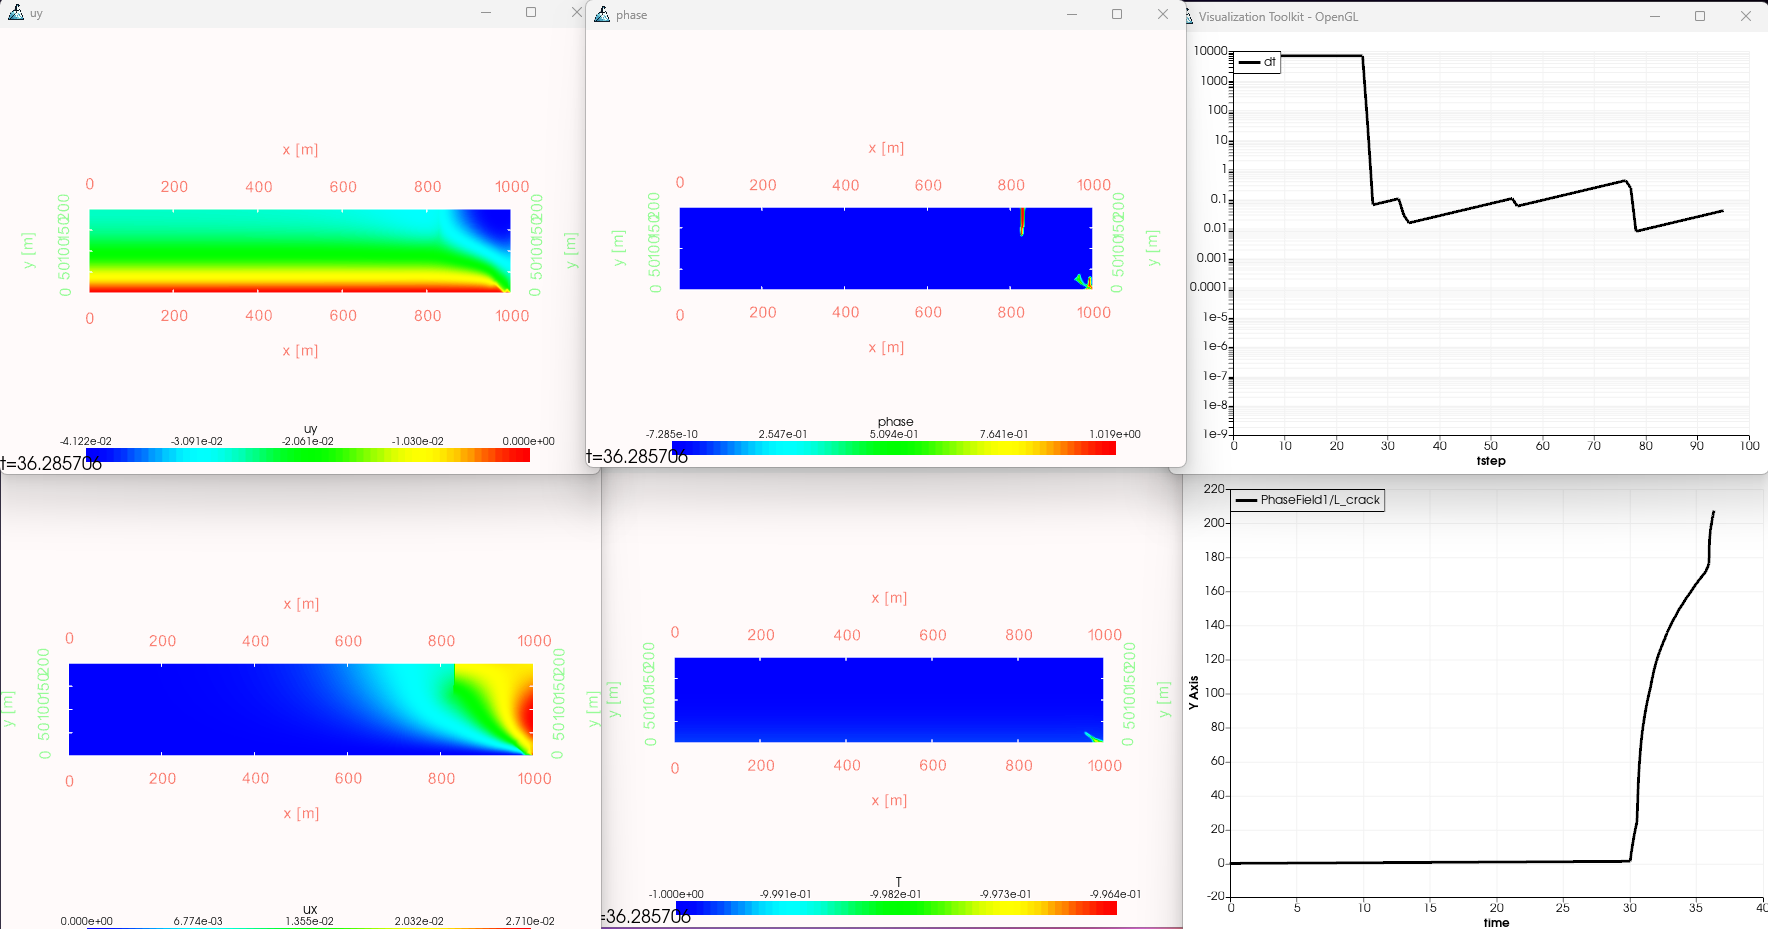
\includegraphics[width=\textwidth]{Screencap_IceCliff_Running.png}
	\caption{Example of figures that open while running the simulation (top left to bottom right): Vertical displacements, phase-field, time increment size vs time increment, horizontal displacement, temperature, and estimated total crack length vs time.}
	\label{fig:Results}
\end{figure}

\subsection{Results while solving}
Once the mesh is generated, run the cliff test case using \textit{mpirun -np 56 ./IceCode TestCases/IceCliffs/IceCliff.json} from the base directory (adapt the number of processes to the amount available, and the generated mesh). During the run, several windows will open, \cref{fig:Results}, showing the state of the system, including surface plots of the phase-field variable, displacements, and temperature. 

\subsection{Post-processing}
While running the simulation, outputs are saved to the \textit{Results} folder, creating:
\begin{itemize}
	\item Backup.hdf5: This file is used for restarting simulations
	\item DofSpace.hdf5: Only used for debugging purposes.
	\item mesh\_0.hdf5: This file contains the mesh information in an easy-to-post-process format. Specifically, it contains the corners of each element and locations of each integration point for which data is saved. 
	\item results\_n.hdf5: These files contain the outputs from the simulation, with n being the output step for which they are saved. Each field is saved can be accessed through its location and name, e.g. accessing the temperature as "internal/T". This file also contains the field "time", indicating to which simulation time the saved results correspond.
	\item TimeData.hdf5: This file contains the global measures: The time, time increment size, crack length, and crack length change. For tri-axial simulations, it also contains the applied displacement and resulting force. 
\end{itemize}

These files use the standard HDF file format \citep{HDF5Group2024}, and therefore can be easily read using a variety of software, including python and MATLAB. Post-processing scripts using MATLAB are included in the test cases' folders, which process the simulations results to animations and figures. For example, running the \textit{TestCases/IceCliffs/PlotData.m} script will create the figures shown in \cref{fig:ResultsPlots}.

\begin{figure}
	\begin{subfigure}{8cm}
		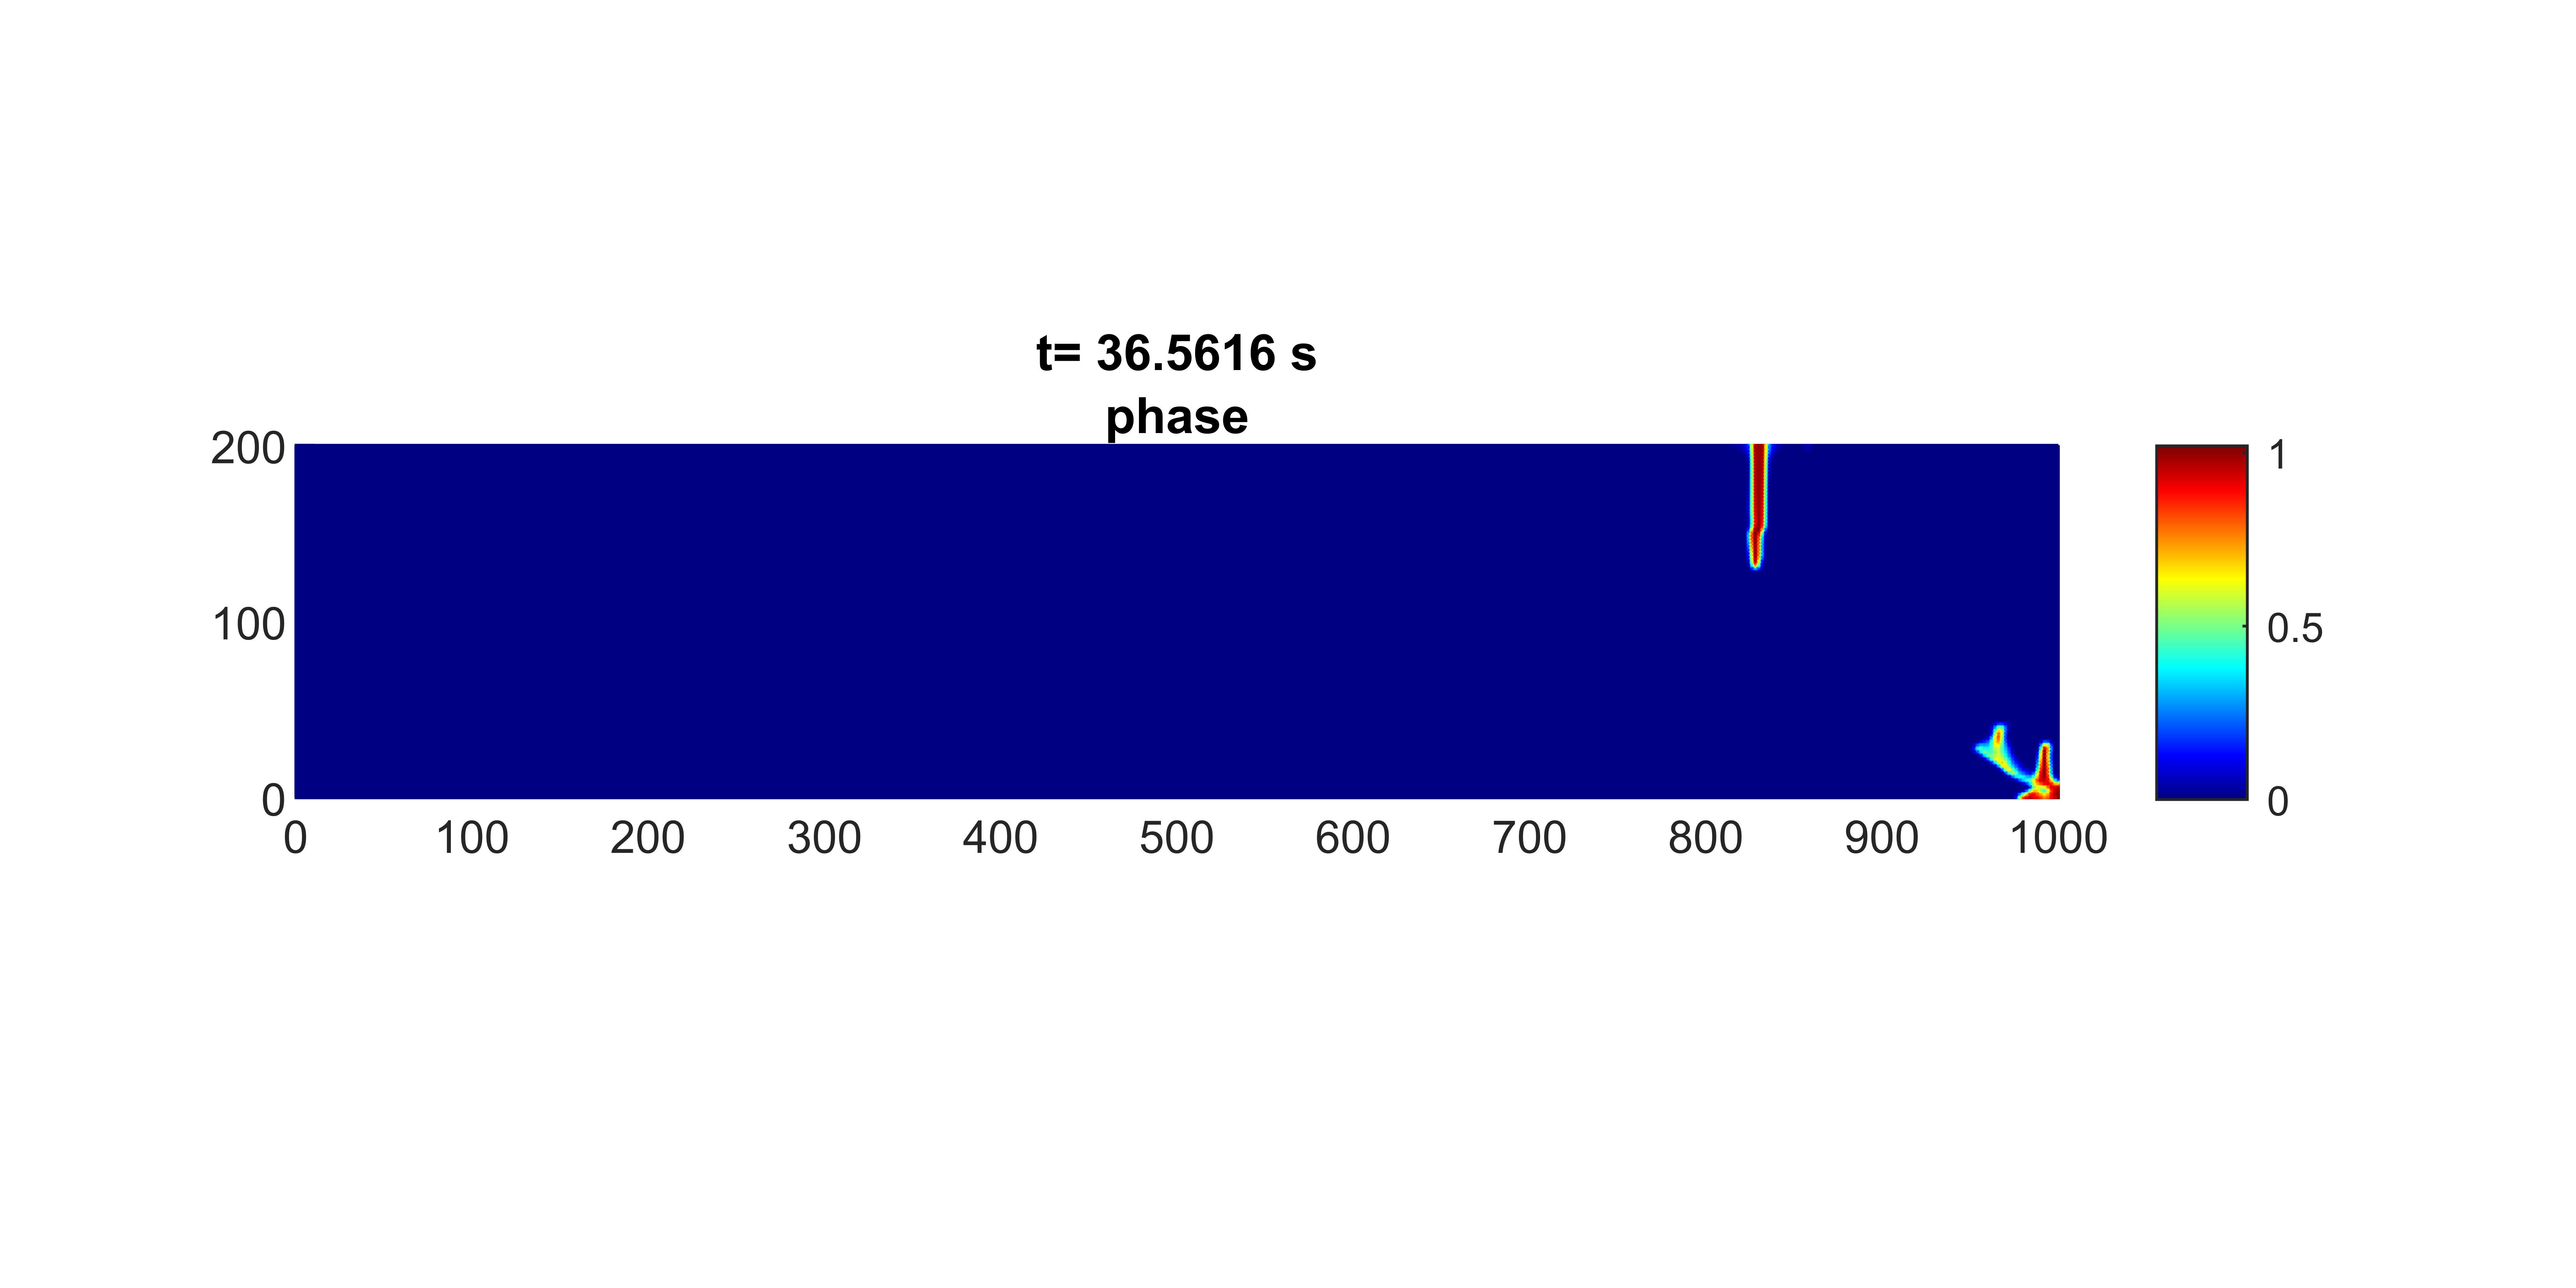
\includegraphics[width=8cm]{../TestCases/IceCliffs/Figures/phase.png}
	\end{subfigure}
	\begin{subfigure}{8cm}
		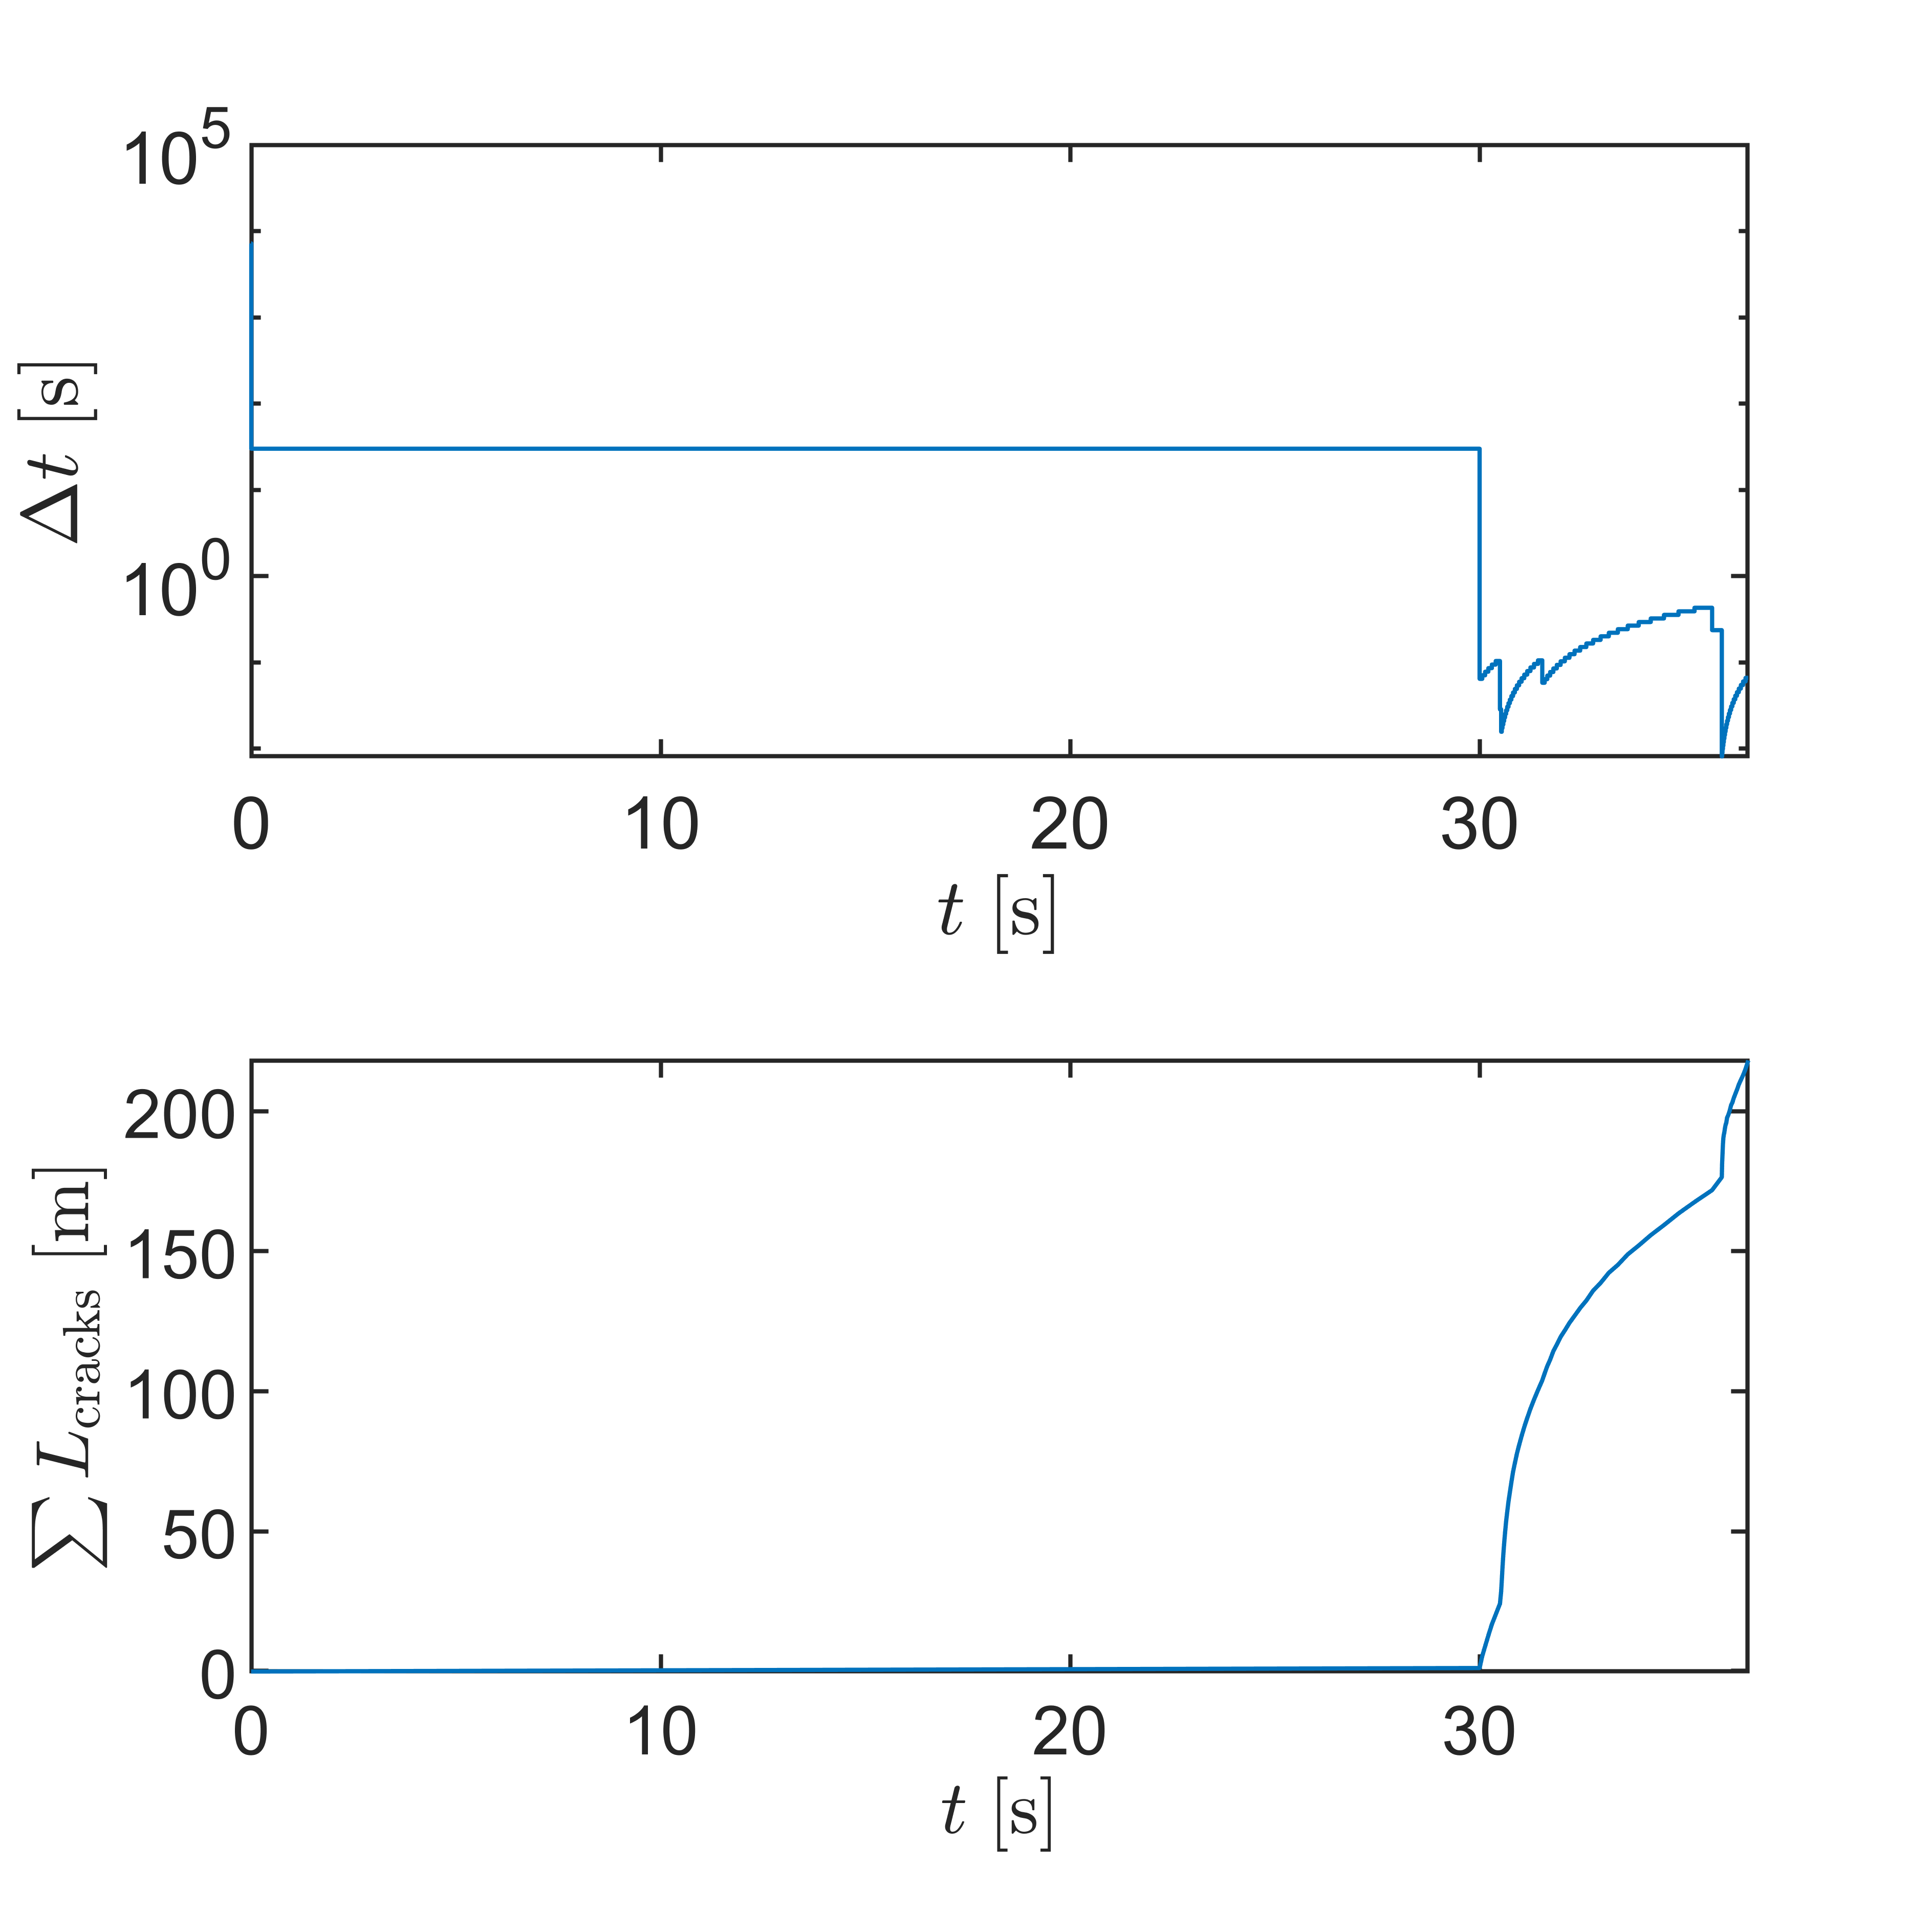
\includegraphics[width=8cm]{../TestCases/IceCliffs/Figures/TimeLFrac.png}
	\end{subfigure}
	\begin{subfigure}{16cm}
		\includegraphics[width=16cm]{../TestCases/IceCliffs/Figures/Stresses.png}
	\end{subfigure}
	\caption{Post-processed results from the ice-cliff failure simulation, showing the phase-field variable at the final time step (top left), the estimated total crack length vs time (top right), and the vertical and horizontal stress at the final time step (bottom).}
	\label{fig:ResultsPlots}
\end{figure}



\FloatBarrier
\section{References}
\renewcommand{\bibsection}{}
\bibliography{references}

\end{document}
